% LTeX: language=es

\chapter{Marco Teórico y Referencial}\label{cap:marcoTeorico}

En este capítulo se realiza una revisión de la literatura y el contexto en el ámbito de la segmentación y tracking de objetos en vídeos, con un enfoque específico en la detección de microgotas. Se analizan las técnicas y algoritmos más relevantes utilizados en este campo, algoritmos clásicos de visión por computador, así como las soluciones basadas en deep learning.

\section {Contextualización de los experimentos analizados}

\subsection{Sprays, aerosoles y nebulizadores}

En este apartado se va a realizar una breve introducción a los sprays, nebulizadores y la técnica de Flow Blurring, que son el contexto en el que se enmarca este trabajo. Se explicará qué son, cómo funcionan y por qué es importante su estudio en el ámbito de la física de fluidos y la microfluídica.

Un \textbf{spray} es un flujo disperso de fase líquida en fase gaseosa, formado por un conjunto de gotas transportadas por el gas, si dichas gotas son finas y estables en suspensión, se denomina \textbf{aerosol}. Los sprays se encuentran en una amplia variedad de aplicaciones, desde la agricultura (aspersores), la medicina (nebulizadores) hasta la industria (inyección de combustible en motores, recubrimiento de superficies). La caracterización de los sprays es fundamental para optimizar su rendimiento y eficiencia, así como para comprender los procesos físicos que ocurren durante su formación y evolución.

Un \textbf{nebulizador} es un dispositivo que transforma un líquido en un aerosol mediante la aplicación de energía, ya sea a través de un flujo de gas, ultrasonidos o vibraciones mecánicas. En la nebulización neumática, el gas aporta energía cinética al líquido, provocando perturbaciones y turbulencias sobre la superficie del líquido, lo que acaba provocando la rotura y formación de gotas. Cabe destacar que este proceso no asegura la esfericidad de las gotas formadas, ya que si el líquido es viscoso se pueden formar filamentos. Por este motivo se descartan el uso de técnicas que asumen la esfericidad de las gotas (p. ej., difracción láser) y se opta por técnicas de visión por computador, que permiten detectar y caracterizar las gotas independientemente de su forma.

\subsection{Flow Blurring}

El nebulizador neumático que se usa en los experimentos analizados en este trabajo son del tipo \textbf{Flow Blurring \cite{ganan2005enhanced}}, desarrollado a partir de 2005 por Gañan Calvo y su grupo de investigación.

La idea física de este tipo de inyector es que la rotura del líquido se produce dentro del inyector por la interacción intensa gas–líquido, que genera recirculación y turbulencia capaces de vencer las fuerzas cohesivas (viscosidad y tensión superficial), formando gotas o filamentos según sean las condiciones. 

\begin{figure}[h] 
    \centering
    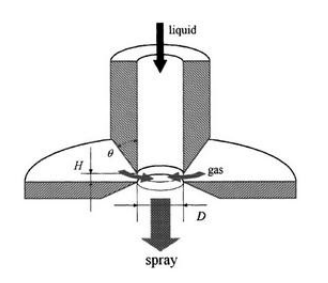
\includegraphics[width=0.6\textwidth]{figures/Inyector2.png}
    \caption{Geometría del Nebulizador Flow Blurring.}
    \label{fig:inyectorEsquema}
\end{figure}

Como se puede observar en la figura \ref{fig:inyectorEsquema}, la geometría se caracteriza con dos magnitudes: la altura $H$ y el diámetro $D$. La relación entre ambas, $\phi = \dfrac{H}{D}$, es un parámetro clave que determina el régimen de nebulización, Flow Focusing o Flow Blurring. Los nebulizadores Flow Blurring poseen una relación $\phi$ menor que $0.5$.

En este tipo de nebulizador neumático, el spray se controla típicamente con presiones ycaudales de gas y líquido. Existe una transferencia de energía (para una presión de gas fija) que se traduce en una presión mínima de líquido capaz de sostener una atomización estable; fuera de esa “ventana” puede aparecer desde spray poco saturado hasta chorro líquido.

\subsection{Obtención de los vídeos de alta velocidad}

Para conseguir captar información de tamaño y velocidades de las gotas se necesita una gran resolución espacial y temporal. Para ello es necesario el uso de cámaras de alta velocidad, en el caso de los experimentos analizados, se ha utilizado una Shimadzu HPV-2 capaz de grabar a 1 millón de fotogramas por segundo (fps). Durante los experimentos se realizan grabaciones cortas de unos 120 frames, variando los intervalos temporales entre frames ($1\mu s$, $2\mu s$, $4\mu s$, ...) y el zoom.

Al aumentar la velocidad de grabación y el zoom, se reduce la cantidad de luz que llega al sensor, lo que hace necesario el uso de un flash de alta intensidad.

El procedimiento de adquisición de los vídeos es el siguiente:
\begin{enumerate}
    \item Montar el sistema de atomización  y posicionar el inyector para capturar en la salida o a una distancia aguas abajo (por ejemplo, 4 cm, mencionada como zona de interés para formación de gotas).
    \item Encender la cámara con antelación (se menciona un calentamiento previo recomendado).
    \item Enfocar usando un patrón (por ejemplo un alambre de diámetro conocido), de forma que el plano enfocado sea el de máxima nitidez.
    \item Repetir enfoque al cambiar el zoom (x1, x3, x6). Este uso del alambre también sirve como calibración geométrica (relación píxel–longitud) si el diámetro del alambre es conocido. 
\end{enumerate}

\vspace*{0,7cm}

\begin{figure}[h] 
    \centering
    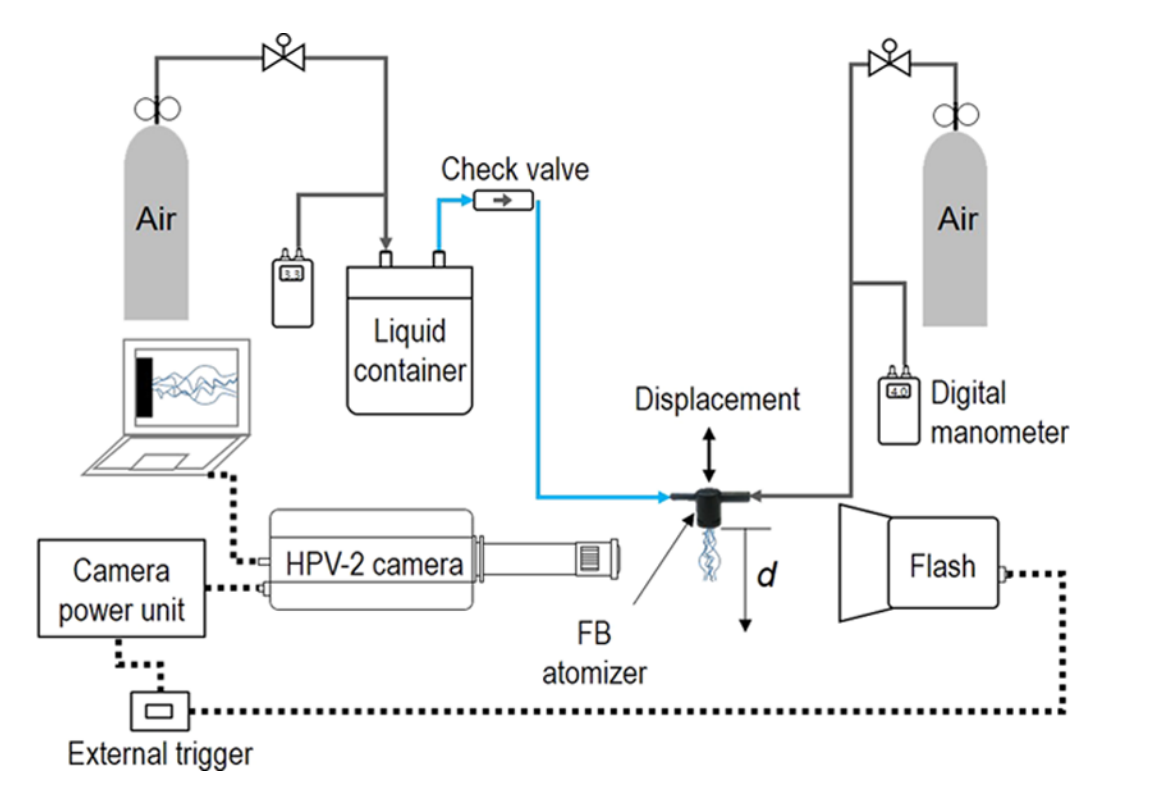
\includegraphics[width=0.8\textwidth]{figures/Exp.png}
    \caption{Montaje experimental para la adquisición de vídeos de alta velocidad.}
    \label{fig:montajeExperimental}
\end{figure}

\section{Introducción al procesamiento de imágenes digitales}\label{sec:intropi}

En esta sección se procederá a dar unas breves pinceladas sobre la representación digital de las imágenes, así como los conceptos básicos del procesamiento de imágenes digitales, que serán necesarios para entender los algoritmos y técnicas que se desarrollarán en los siguientes apartados. Se explicará qué es una imagen digital, cómo se representa y cuáles son las operaciones básicas que se pueden realizar sobre ella.

En este proyecto se trabaja con vídeos de alta velocidad, que no son más que secuencias de imágenes digitales relacionadas temporalmente. Por lo tanto, es fundamental entender cómo se representan las imágenes digitales para poder aplicar técnicas de procesamiento de imágenes y análisis de vídeo.

\subsection{¿Qué es una imagen digital?}

Las imágenes se pueden dividir principalmente en dos tipos: imágenes analógicas e imágenes digitales. Las imágenes analógicas son una representación física de la luz, en la fotografía tradicional, por ejemplo, la luz reacciona con sustancias químicas para formar una imagen. Esta variación química es continua, lo que significa que las transiciones de color o luz fluyen sin interrupciones, formando un gradiente suave sin divisiones exactas. Por otro lado, las imágenes digitales son una representación discreta de la luz, dónde la imagen se divide en una cuadrícula de pequeños elementos numéricos llamados píxeles. Cada píxel tiene un valor que representa la intensidad de la luz (en imágenes en escala de grises) o los valores de color (en imágenes a color). Esta representación discreta permite almacenar, procesar y analizar las imágenes utilizando algoritmos computacionales, como es el caso.

\subsection{Representación de las imágenes digitales}

Para representar una imagen digital, se utiliza una matriz de píxeles. Definamos $p = f(x, y)$, donde $x$ y $y$ son las coordenadas espaciales y $f$ es la función de iluminación que asigna un valor de intensidad (o color) a cada píxel. En el caso de imágenes en escala de grises, cada píxel tiene un valor que representa la intensidad de la luz, típicamente en un rango de 0 a 255, donde 0 representa el negro y 255 representa el blanco. En el caso de imágenes a color, cada píxel se representa mediante tres valores (R, G, B), cada uno en un canal (matriz) diferente que corresponden a las intensidades de los colores rojo, verde y azul, respectivamente \cite{gonzalez2018digital}.

Así que para una imagen digital de tamaño $n x n$, la representación en formato matricial $A$ sería la siguiente:

\begin{equation} \label{eq:matriz}
\mathbf{A} = 
\begin{bmatrix}
f(0,0) & f(0,1) & \dots & f(0,n-1) \\
f(1,0) & f(1,1) & \dots & f(1,n-1) \\
\vdots & \vdots & \ddots & \vdots \\
f(n-1,0) & f(n-1,1) & \dots & f(n-1,n-1)
\end{bmatrix}
\end{equation}

O representada de manera compacta:

\begin{equation} \label{eq:matrizCompacta}
P_{i,j} = f(i, j) ~~~~ i,j \in {0, n-1}
\end{equation}

Una vez definido la forma de representar imágenes digitales, podemos proceder a explicar algunas técnicas clásicas de procesamiento.

\section{Técnicas clásicas}

En este apartado de abordarán de manera teórica los algoritmos y técnicas que se han tenido en cuenta para el desarrollo de este proyecto, iremos desde el preprocesamiento, pasando por la segmentación, operaciones morfológicas y finalmente el tracking de objetos, cubriendo así todo el pipeline de la solución implementada.

\subsection{Preprocesamiento de imágenes}\label{subsec:preproc}

El preprocesamiento de imágenes es una etapa fundamental en el procesamiento de imágenes digitales, ya que permite mejorar la calidad de la imagen y facilitar la posterior segmentación y análisis. En esta sección se describirán las técnicas de reducción de ruido y mejora de contraste que se han considerado para el desarrollo de este proyecto.

\subsubsection{Mejora del contraste}
La idea detrás de la mejora del contraste es aumentar la diferencia entre las intensidades de los píxeles, o lo que es lo mismo, hacer más oscuro lo oscuro y más claro lo claro. Ya que si los frames presentan un histograma de intensidades concentrado en un rango pequeño, la segmentación e identificación de detalles puede resultar difícil. Para solventar este problema se han tenido en cuenta las siguientes técnicas:

\textbf{Ecualización Adaptativa del Histograma con Contraste Limitado (CLAHE):} La ecualización global del histograma puede amplificar el ruido en regiones uniformes, ya que un histograma muy concentrado en pocos valores se estira de forma agresiva al redistribuirse. Por eso, la idea principal de CLAHE \cite{zuiderveld1994clahe} es dividir la imagen en pequeñas regiones (tiles) y aplicar la ecualización del histograma de manera local en cada una de ellas. Además, para evitar la sobreamplificación del ruido, el histograma de cada tile se recorta en un límite de contraste configurable (clip limit), y el exceso se redistribuye uniformemente sobre el resto del histograma. Si no existiese este límite, el ruido se podría amplificar excesivamente; por ejemplo, si una zona de la imagen es homogénea (p.\,ej., un fondo oscuro) y contiene un par de píxeles ruidosos, tras la ecualización esos píxeles, antes imperceptibles, se convertirían en puntos brillantes. Finalmente, para evitar costuras visibles en las fronteras entre tiles, los valores de píxeles cercanos a los bordes se obtienen mediante interpolación bilineal entre los tiles vecinos, logrando así una transición suave y continua.

\textbf{Estiramiento de contraste:} La idea detrás de esta técnica es remapear los valores de intensidad de la imagen al rango completo de valores posibles (0-255 para imágenes en escala de grises). Es decir, hace una transformación lineal que asigna el percentil mínimo ($p_{min}$) de intensidad a 0 y el percentil máximo ($p_{max}$) a 255, estirando proporcionalmente los valores intermedios:

\begin{equation}
I'(x,y) = \frac{I(x,y) - p_{min}}{p_{max} - p_{min}} \cdot 255
\end{equation}

Donde $I(x,y)$ es la intensidad original del píxel en la posición $(x,y)$, y $I'(x,y)$ es la intensidad remapeada. La razón para usar los percentiles en lugar de los valores mínimo y máximo absolutos es que si se usa el mínimo y máximo absolutos, un solo píxel ruidoso extremo puede arruinar el resultado. Por ejemplo, si hay un único píxel con valor 10 y otro con valor 250 por ruido, el estiramiento apenas hace nada porque el rango ya parece amplio. En cambio, usando percentiles (p.\,ej., el 1\% y el 99\%), se ignoran esos valores extremos y se obtiene un estiramiento más representativo del rango real de intensidades en la imagen.

\begin{figure}[p]
    \centering
    \small
    
    \begin{subfigure}[b]{0.32\textwidth}
        \centering
        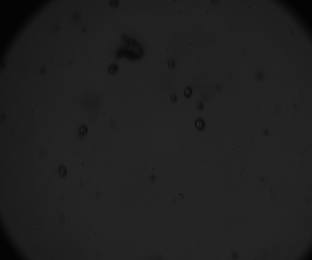
\includegraphics[width=\textwidth]{figures/1_img_original.jpg}
        \caption{Imagen Original (Grises)}
        \label{fig:img_orig}
    \end{subfigure}
    \hfill
    \begin{subfigure}[b]{0.55\textwidth}
        \centering
        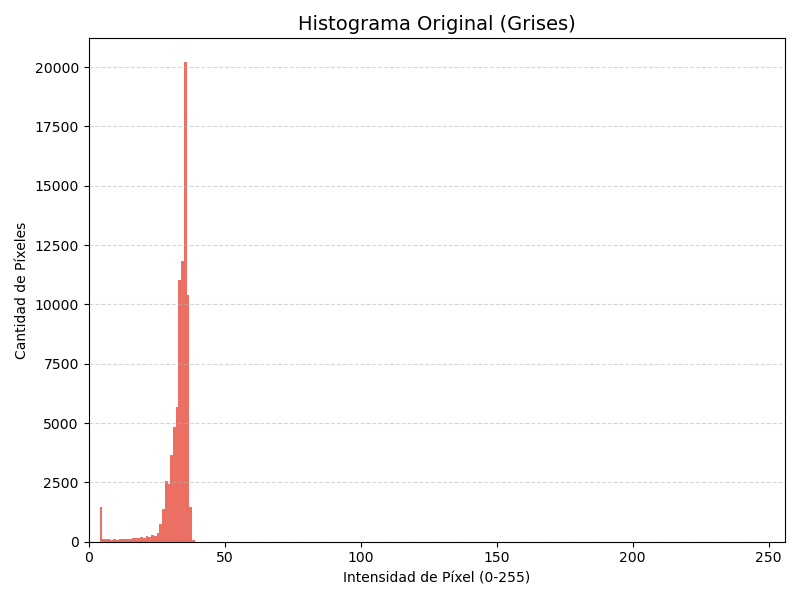
\includegraphics[width=\textwidth]{figures/1_hist_original.png}
        \caption{Histograma Original}
        \label{fig:hist_orig}
    \end{subfigure}
    
    \vspace{0.3cm}
    
    \begin{subfigure}[b]{0.32\textwidth}
        \centering
        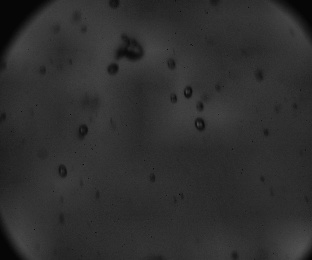
\includegraphics[width=\textwidth]{figures/2_img_clahe.jpg}
        \caption{Imagen con CLAHE}
        \label{fig:img_clahe}
    \end{subfigure}
    \hfill
    \begin{subfigure}[b]{0.55\textwidth}
        \centering
        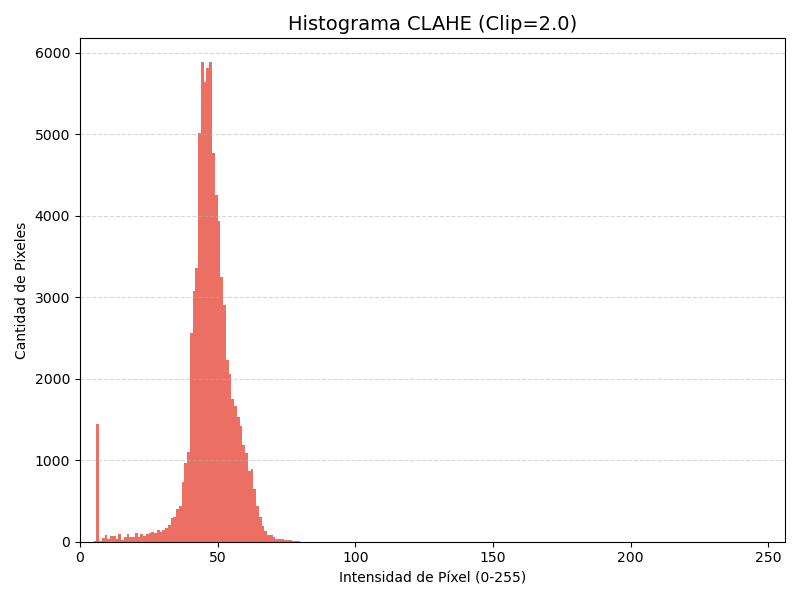
\includegraphics[width=\textwidth]{figures/2_hist_clahe.png}
        \caption{Histograma CLAHE}
        \label{fig:hist_clahe}
    \end{subfigure}
    
    \vspace{0.3cm} 
    
    \begin{subfigure}[b]{0.32\textwidth}
        \centering
        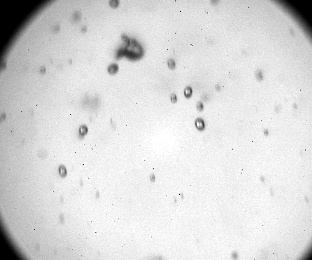
\includegraphics[width=\textwidth]{figures/3_img_estiramiento.jpg}
        \caption{Imagen con Estiramiento}
        \label{fig:img_estir}
    \end{subfigure}
    \hfill
    \begin{subfigure}[b]{0.55\textwidth}
        \centering
        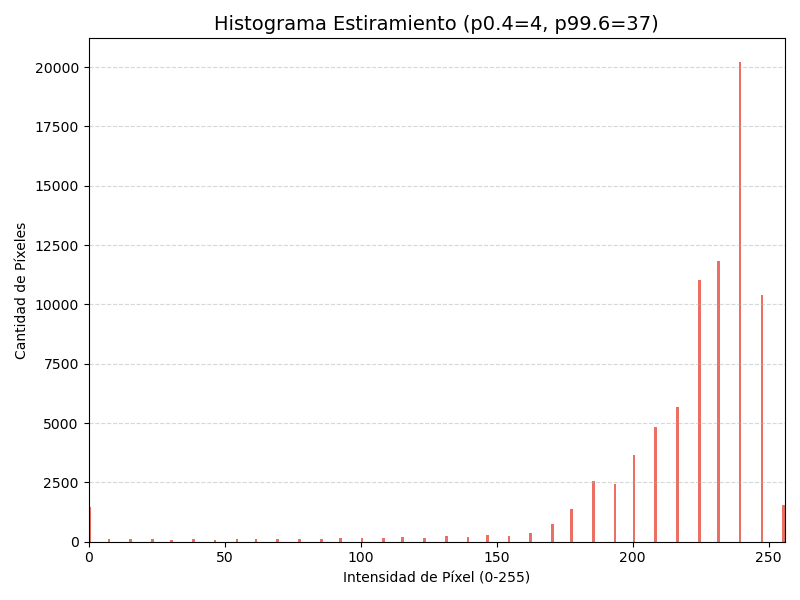
\includegraphics[width=\textwidth]{figures/3_hist_estiramiento.png}
        \caption{Histograma Estiramiento}
        \label{fig:hist_estir}
    \end{subfigure}
    
    \caption{Comparativa de técnicas de mejora: (a-b) Imagen original de bajo contraste; (c-d) Resultado tras aplicar ecualización adaptativa local (CLAHE); (e-f) Resultado tras estiramiento lineal de histograma mediante percentiles.}
    \label{fig:mosaico_histogramas}
\end{figure}

En la figura \ref{fig:mosaico_histogramas} se puede observar un ejemplo de cómo el histograma de la imagen original (con bajo contraste) se concentra en un rango estrecho de intensidades, mientras que tras aplicar CLAHE o estiramiento de contraste, el histograma se distribuye de manera más uniforme a lo largo del rango completo, lo que mejora la visibilidad de los detalles en la imagen.

\subsubsection{Reducción de ruido}

Los procesos de mejora de contraste, especialmente el estiramiento por percentiles, pueden introducir o amplificar ruido de tipo sal y pimienta. Para eliminarlo sin degradar los bordes de las gotas se han considerado los siguientes enfoques:

\paragraph{Filtros de suavizado clásicos:} Uno de los los filtros más comunes en el procesamiento de imágenes es el \textbf{filtro gaussiano}, que convoluciona la imagen con un núcleo gaussiano ($G(x,y,\sigma)$), atenuando las zonas donde hay cambios bruscos de intensidad (como el ruido). El parámetro $\sigma$ controla el grado de suavizado, siendo un valor más alto sinónimo de mayor suavizado. La fórmula que define el peso de cada píxel del núcleo de la convolución es la siguiente:
\begin{equation}
G(x,y,\sigma) = \frac{1}{2\pi\sigma^2} e^{-\frac{x^2 + y^2}{2\sigma^2}}
\end{equation}
En otras palabras, el filtro gaussiano asigna pesos más altos a los píxeles cercanos al centro del núcleo y pesos más bajos a los píxeles más alejados, lo que resulta en un efecto de suavizado que preserva las estructuras generales de la imagen mientras reduce el ruido.
Otro filtro común es el \textbf{filtro de mediana}, que reemplaza cada píxel con la mediana de los valores de los píxeles en su vecindad. Este filtro es especialmente efectivo para eliminar el ruido de tipo sal y pimienta, ya que la mediana no se ve afectada por valores extremos (píxeles ruidosos), a diferencia del promedio que sí puede ser influenciado por ellos.

\paragraph{Fast Non-Local Means Denoising (fNLM):} Los filtros clásicos solo consideran la información de los píxeles cercanos, pero el algoritmo \textbf{fNLM} \cite{ipol.2011.bcm_nlm} asume que una imagen puede tener patrones repetitivos como texturas o zonas lisas, así que toma información de todos los píxeles de la imagen para el suavizado. El algoritmo trabaja con ventanas de píxeles (patches), es decir el algoritmo cogerá una ventana alrededor del píxel a suavizar (el parche $v(N(i))$) y buscará en toda la imagen ventanas similares ($v(N(j))$). La definición matemática es la siguiente:
\begin{equation}
    NL(v) = \frac{1}{C(i)} \sum_{j \in \Omega} e^{-\frac{||v(N_i) - v(N_j)||^2_{2,a}}{h^2}} v(j)
\end{equation}
Donde $NL(v)$ es el nuevo valor que le vamos a dar al píxel $i$, $C(i)$ es un factor de normalización, se divide por la suma total de los pesos. El $\sum_{j \in \Omega} ... v(j)$ Es la suma de los valores de los píxeles $j$ multiplicados por un peso que explicaremos a continuación. $||v(N_i) - v(N_j)||^2_{2,a}$ mide la similitud entre los parches, es decir, la distancia euclídea entre los parches $N_i$ y $N_j$, ponderada por una función gaussiana que da más importancia a los píxeles cercanos al centro del parche. El parámetro $h$ controla el grado de suavizado, siendo un valor más alto sinónimo de mayor suavizado. Esto hace que si el parche $N_j$ es muy similar al parche $N_i$, el peso será alto y el valor de $v(j)$ contribuirá significativamente al nuevo valor de $i$. Por el contrario, si el parche $N_j$ es diferente, el peso será bajo y su contribución será mínima. De esta forma, el algoritmo logra reducir el ruido mientras preserva los detalles y texturas de la imagen. Este algoritmo es fast ya que se restringe la búsqueda de parches similares a una ventana de tamaño $S$ alrededor del píxel $i$, en lugar de buscar en toda la imagen, lo que reduce el orden de complejidad de  $\mathcal{O}(N^2)$ a $\mathcal{O}(N \log N)$, donde $N$ es el número total de píxeles en la imagen.


\subsection{Segmentación de imágenes}\label{subsec:segmentacion}

Segmentación es el proceso de dividir una imagen en regiones o segmentos con significado semantico, en este caso, el objetivo es segmentar las gotas del fondo.

\subsubsection{Umbralización}

La umbralización es una de las técnicas de segmentación más simple, consiste en convertir una imagen en escala de grises en una imagen binaria, donde los píxeles se clasifican como pertenecientes a un objeto (en este caso, una gota) o al fondo, dependiendo de si su intensidad es mayor o menor que un umbral $T$.

En la umbralización global, se elige un único valor de $T$ para toda la imagen. El método \textbf{Otsu} \cite{otsu1979} selecciona automáticamente el umbral que maximiza la varianza entre las clases:
\begin{equation}
    T^{*} = \arg\max_T \left[ w_{0}(T)w_{1}(T)(\mu_{0}(T)-\mu_{1}(T))^2\right]
\end{equation}
Donde $w_{0}(T)$ y $w_{1}(T)$ son las proporciones de las clases de fondo y objeto respectivamente, y $\mu_{0}(T)$ y $\mu_{1}(T)$ son las medias de intensidad de cada clase. Sin embargo, en imágenes con iluminación no uniforme o bajo contraste, la umbralización global puede no ser efectiva, ya que un único umbral puede no separar adecuadamente los objetos del fondo en todas las regiones de la imagen.

Para solucionar este problema, se ha optado por la \textbf{umbralización adaptativa}, en concreto, su versión gaussiana, que calcula un umbral local $T(x,y)$
para cada píxel basado en la media ponderada gaussiana de los píxeles vecinos en una ventana de tamaño $N$ centrada en $(x,y)$, a la que se le resta una constante $C$ para ajustar el umbral:
\begin{equation}
    T(x,y) = \mu_{gauss}(x, y) - C
\end{equation}
El uso de un umbral local asegura la robustez de la segmentación frente a variaciones de iluminación.

\subsubsection{Extracción de contornos}
Una vez binarizada la imagen, los contornos permiten delimitar exactamente cada región segmentada. El algoritmo de \textbf{Suzuki \& Abe} \cite{SUZUKI198532} realiza un recorrido topológico de la imagen binaria etiquetando los bordes exteriores e interiores mediante una única pasada sobre los píxeles, lo que lo hace eficiente en memoria y tiempo. OpenCV expone este algoritmo a través de \texttt{cv2.findContours}, con distintos modos de recuperación (\texttt{RETR\_EXTERNAL} para contornos solo externos, \texttt{RETR\_TREE} para la jerarquía completa) y métodos de aproximación (\texttt{CHAIN\_APPROX\_SIMPLE} para comprimir segmentos rectos, \texttt{CHAIN\_APPROX\_NONE} para devolver todos los puntos).

\subsection{Operaciones morfológicas}

Las operaciones morfológicas operan sobre conjuntos binarios, mediante un elemento estrcuturante (normalmente un cuadrado o un círculo) de forma y tamaño configurable. Las dos operaciones básicas son la dilatación y la erosión, que forman las operaciones compuestas. La \textbf{erosión} elimina píxeles de los bordes de los objetos, lo que puede ayudar a eliminar pequeñas regiones ruidosas o separar objetos conectados. Por otro lado, la dilatación agrega píxeles a los bordes de los objetos, lo que puede ayudar a cerrar pequeños agujeros o conectar objetos cercanos. Combinando estas dos operaciones se puede obtener la apertura y el cierre.

La \textbf{apertura} (opening) es la combinación de erosión seguida de dilatación, lo que elimina objetos más pequeños que el kernel y suaviza los bordes de los objetos más grandes, se suele usar para eliminar ruido del tipo sal y pimienta:
\begin{equation}
 A \circ B = (A \ominus B) \oplus B
\end{equation}
El \textbf{cierre} (closing) es la combinación de dilatación seguida de erosión, lo que cierra pequeños agujeros dentro de los objetos y conecta objetos cercanos, se suele usar para rellenar huecos en los objetos segmentados:
\begin{equation}
 A \bullet B = (A \oplus B) \ominus B
\end{equation}
En la implementación desarrollada se aplica primero la apertura para eliminar el ruido generado por la umbralización, y a continuación el cierre para recuperar la integridad de las gotas que hubieran quedado fragmentadas.

\subsection{Tracking de objetos}

El tracking o seguimiento de objetos en vídeos es el proceso de asociar, frame a frame, las detecciones correspondientes al mismo objeto, construyendo así su trayectoria.

\subsubsection{Flujo óptico de Lucas-Kanade}

El algoritmo de \textbf{Lucas-Kanade} \cite{lucas1981iterative} se basa en la hipótesis de constancia de intensidad, es decir, asume que la intensidad de los píxeles de un objeto se mantiene constante entre frames consecutivos. Para ello, toma una ventana local de píxeles alrededor de cada punto de interés y asume que todos los píxeles de dicha ventana se desplazan de forma uniforme. A continuación, busca en el siguiente frame la posición que minimiza la diferencia de intensidades respecto a la ventana original, obteniendo así el vector de desplazamiento del punto.
Matemáticamente, el algoritmo resuelve la siguiente ecuación para cada punto de interés:
\begin{equation}
    \begin{pmatrix} \sum I_x^2 & \sum I_x I_y \\ \sum I_x I_y & \sum I_y^2 \end{pmatrix}
    \begin{pmatrix} u \\ v \end{pmatrix}
    =
    -\begin{pmatrix} \sum I_x I_t \\ \sum I_y I_t \end{pmatrix}
\end{equation}

donde $(u, v)$ es el vector de desplazamiento que se desea calcular, $I_x$ e $I_y$ son las derivadas parciales de la intensidad de la imagen respecto a $x$ e $y$, respectivamente, y $I_t$ es la derivada parcial respecto al tiempo, es decir, la diferencia de intensidades entre los dos frames.

Este sistema es sobredeterminado: la ecuación básica del flujo óptico $I_x u + I_y v + I_t = 0$ tiene dos incógnitas ($u$ y $v$) pero se aplica a todos los píxeles de la ventana local, generando más ecuaciones que incógnitas. Para obtener una solución única, Lucas-Kanade minimiza la suma de los errores al cuadrado de todas las ecuaciones de la ventana, lo que conduce al sistema matricial $2\times2$ mostrado anteriormente, que sí tiene solución única siempre que la matriz del sistema no sea singular, es decir, siempre que exista suficiente textura en la ventana local.

Sin embargo, la formulación básica falla cuando el desplazamiento entre frames es grande en comparación con el tamaño de la ventana, ya que la hipótesis de desplazamiento uniforme deja de ser válida. Para solventar esto, en la práctica se emplea la \textbf{versión piramidal} del algoritmo \cite{bouguet2001pyramidal}: la imagen se submuestrea en varios niveles de resolución formando una pirámide, se calcula el flujo en el nivel más grueso (donde los grandes desplazamientos se convierten en pequeños) y el resultado se refina progresivamente hacia la resolución original. OpenCV implementa esta variante a través de la función \texttt{cv2.calcOpticalFlowPyrLK}, que es la utilizada en la implementación desarrollada.

\subsubsection{Asignación por distancia mínima}

Una vez predichas las posiciones futuras de los tracks activos mediante flujo óptico, el problema de asociación consiste en decidir qué detección del fotograma actual corresponde a cada track. La estrategia greedy por distancia mínima selecciona para cada detección el track disponible más cercano en términos de distancia euclídea entre centroides, siempre que dicha distancia no supere un umbral máximo configurable. Los tracks que no reciben ninguna detección durante varios fotogramas consecutivos se consideran perdidos y se descartan, mientras que las detecciones sin track asignado generan nuevos tracks.
Este enfoque, combinado con la predicción de Lucas-Kanade, es suficientemente robusto para los vídeos analizados de corta duración ( $\approx$ 120 fotogramas) y con movimiento de gotas relativamente uniforme sin necesidad de recurrir a métodos más complejos como el filtro de Kalman.

\section{Técnicas basadas en deep learning}

Además de los algoritmos clásicos descritos anteriormente, se evaluó la viabilidad de utilizar modelos de segmentación basados en aprendizaje profundo, en particular el modelo \textbf{Segment Anything Model (SAM)} \cite{kirillov2023sam}. SAM es un modelo de segmentación de propósito general entrenado sobre más de mil millones de máscaras anotadas, capaz de segmentar cualquier objeto a partir de prompts en forma de puntos, cajas delimitadoras o máscaras previas. Su arquitectura combina un codificador de imagen basado en \textbf{Vision Transformer (ViT)} con un decodificador ligero de máscaras, lo que le permite generar segmentaciones precisas en una amplia variedad de dominios sin necesidad de reentrenamiento.

Sin embargo, tras las pruebas realizadas en el entorno local, se decidió descartar el uso de SAM como solución final por las siguientes razones: el modelo requiere una GPU con memoria suficiente y una instalación de CUDA, lo que supone una barrera de hardware para los investigadores del departamento. Los tiempos de inferencia por fotograma son significativamente mayores que los de la solución clásica y, en las pruebas realizadas, la ventaja en precisión de segmentación no justificaba el sobrecoste computacional para el tipo de imágenes analizadas, donde las gotas presentan un contraste razonablemente bien definido tras el preprocesamiento. Por estos motivos, se optó por la solución clásica basada en OpenCV, que ofrece un buen equilibrio entre precisión, rendimiento y accesibilidad.